\documentclass[12pt,a4paper]{article}
\usepackage[round]{natbib}
\usepackage{amsmath}
\usepackage{amssymb}
\usepackage{amsthm}
\usepackage{amsfonts}
\usepackage{graphicx}
\usepackage[utf8]{inputenc}
\usepackage[english]{babel}
\usepackage[all]{xy}
\usepackage{float}
\usepackage{tikz}
\usepackage{verbatim}
\usepackage[left=2cm,right=2cm,top=2cm,bottom=2cm]{geometry}
\usepackage[hidelinks]{hyperref}
\usepackage{caption}
\usepackage{subcaption}
\usepackage{psfrag}

\usepackage[T1]{fontenc} % Output font encoding for international characters

%\usepackage{mathpazo} % Palatino font

\newtheorem{thm}{Theorem}
\newtheorem{lem}[thm]{Lemma}
\newtheorem{defn}[thm]{Definition}
\newtheorem{definition}{Definition}[section] 
\newtheorem{theorem}{Theorem}
\newtheorem{exa}[thm]{Example}
\newtheorem{rem}[thm]{Remark}
\newtheorem{coro}[thm]{Corollary}
\newtheorem{quest}{Question}[section]

\newcommand{\N}{\mathbb{N}}
\newcommand{\Z}{\mathbb{Z}}
\newcommand{\Q}{\mathbb{Q}}
\newcommand{\R}{\mathbb{R}}
\newcommand{\C}{\mathbb{C}}

\begin{document}
	
	%----------------------------------------------------------------------------------------
	%	TITLE PAGE
	%----------------------------------------------------------------------------------------
	
	\begin{titlepage} % Suppresses displaying the page number on the title page and the subsequent page counts as page 1
		
		\newcommand{\HRule}{\rule{\linewidth}{0.5mm}} % Defines a new command for horizontal lines, change thickness here
		
		\center % Centre everything on the page
		
		%------------------------------------------------
		%	Headings
		%------------------------------------------------
		
		\textsc{\LARGE Boise State University}\\[1.5cm] % Main heading such as the name of your university/college
		
		\textsc{\Large BSU}\\[0.5cm] % Major heading such as course name
		
		\textsc{\large Final Project}\\[0.5cm] % Minor heading such as course title
		
		%------------------------------------------------
		%	Title
		%------------------------------------------------
		
		\HRule\\[0.4cm]
		
		{\huge\bfseries INVERSE METHODS FOR  SHALLOW WATER  EQUATIONS }\\[0.4cm] % Title of your document
		
		\HRule\\[1.5cm]
		
		%------------------------------------------------
		%	Author(s)
		%------------------------------------------------
		
		\begin{minipage}{0.4\textwidth}
			\begin{flushleft}
				\large
				\textit{Author}\\
				 \textsc{Brian KYANJO} % Your name
			\end{flushleft}
		\end{minipage}
		~
		\begin{minipage}{0.4\textwidth}
			\begin{flushright}
				\large
				\textit{Supervisor}\\
				Prof. Jodi\textsc{~Mead} % Supervisor's name
			\end{flushright}
		\end{minipage}
		
		% If you don't want a supervisor, uncomment the two lines below and comment the code above
		%{\large\textit{Author}}\\
		%John \textsc{Smith} % Your name
		
		%------------------------------------------------
		%	Date
		%------------------------------------------------
		
		\vfill\vfill\vfill % Position the date 3/4 down the remaining page
		
		{\large\today} % Date, change the \today to a set date if you want to be precise
		
		%------------------------------------------------
		%	Logo
		%------------------------------------------------
		
		%\vfill\vfill
		\includegraphics[width=0.2\textwidth]{"Screenshot 2021-03-19 at 10.18.39 PM"}\\[1cm] % Include a department/university logo - this will require the graphicx package

		%----------------------------------------------------------------------------------------
		
		\vfill % Push the date up 1/4 of the remaining page
		
	\end{titlepage}
	
	%----------------------------------------------------------------------------------------
	\section*{Abstract}
	\tableofcontents
	\newpage
	\section{Introduction}
	\subsection{Background}
	The shallow water  equations (SWE) are a system of hyperbolic partial differential equations (PDEs) describing the flow below a pressure surface in a fluid. They have been frequently used to model several real-life problems i.e. the propagation of tsunamis waves in the ocean \citep{dias2007dynamics} and modeling of atmospheric turbulence. Deep knowledge is required to handle such events, therefore first, robust, and computationally efficient methods like inverse methods are required to solve the shallow water equations.
	
	\subsection{General Objectives}
	
	\begin{itemize}
	\item To discover a best approach of chosing an initial guess ($m_0$) for the SWE problem while  recovering true estimates ($m_{true}$).
	\item  To verify if the confidence interval of the recovered estimates captures the true parameter estimates.
	\item To check the relationship between the recovered estimates.
	\item  To investigate how the order of the roughening matrix impact the $\chi^2$, p-value and L2-norm of the recovered estimates.
\end{itemize}


	\subsection{Literature}
		Inverse methods  have been frequently used to handle shallow water problems; for instance   \citet{cit} proposed technique which reconstructed the initial tsunami waveform using inversion of the remote measurements of the water level data. \citet{monnier2016inverse}, \citet{gessese2012direct}, and \citet{voronina2013inverse}.
	
	
	\section{ Problem Formulation and Methods}
 \subsection{Formulation of  the Forestclaw code}
 
 \subsubsection{Riemann solvers}
 Riemann solvers are numerical methods in which time-averaged fluxes of all conserved quantities are calculated to solve fundamental problems in conservation laws named Riemann problems.   A Riemann problem can be defined as a specific initial value problem  (Cauchy) of a partial differential equation (PDE) that consists of conservation equations \eqref{rp0}  combined with piece-wise constant initial data which has a single discontinuity in the domain of interest as shown in equation \eqref{rp}  \citep{ge:2011}. 
 \begin{eqnarray}
 	q_{t} + f(q)_{x}& =& 0
 	\label{rp0}\\
 	q(x,0)& =& \begin{cases}
 		q_{L}, & \text{if \, $x \le 0,$}\\
 		q_{R},& \text{if \, $x > 0,$}\\
 		
 	\end{cases}  
 	\label{rp}     
 \end{eqnarray}
 where $f(q)_{x} \in \mathbb{R}^{m}$ is a vector of conserved quantities,  $q_{R}$ and $q_{L}$ are two piece-wise constant states separated by a discontinuity. 
 
 \subsubsection{Shallow Water Equations (SWE)}
 The SWE are a system of hyperbolic PDEs governing the flow below a pressure surface in a fluid. They arise from the Navier-Stokes equations.  In one dimension, the SWE  can be used to model a fluid in a channel of unit width, taking the vertical velocity negligible, and horizontal velocity roughly constant throughout any cross section of the channel  \citep{ge:2008}.  \\
 
 Consider small-amplitude waves in a one-dimensional fluid channel that is shallow relative to its wavelength. The conservation of momentum equation is written in terms of pressure, $p(x,t) = \frac{1}{2} gh^{2}$, and the height field $h(x,t)$ ($m$), which breaks down into system \eqref{p12}.
 
 \begin{equation}
 	\begin{aligned}
 		h_{t} + (hu)_x &= 0 \\
 		(hu)_t + \left(hu^{2} + \frac{1}{2} gh^{2} \right)_x & = 0 
 	\end{aligned}
 	\label{p12}
 \end{equation}	
 where $hu$ measures the flow rate of water past a point,  $\rho$ ($kg/m^3$) is the constant density of the in-compressible fluid, and $u(x,t)$ ($m/s$) is the horizontal velocity. \\
 
 A very simple set of initial conditions is a single discontinuity at the middle of the channel.  In this case, we set $h$ and $hu$ equal to constants on either side of the channel.  This problem is a classic Riemann Problem, and for the SWE, has an exact solution.  We assume the discontinuity is at $x = 0$. 
 The variation of $h$ and $hu$ on either side of the discontinuity leads the waves in the Riemann problem to move at different speeds creating discontinuities (shocks) or changing regions (rarefactions) \citep{leveque2002finite}.  At $x = 0$ and $t = 0$,   the discontinuity is located between the left and right state, so the solution at the left ($q_{l}$)and right($q_{r}$) states are given by: 

\begin{equation}
	q_{l} = [ h_l, \, u_l, \, hu_l]^T \quad \text{and} \quad  q_{r} = [ h_r, \, u_r, \, hu_r]^T
		\label{ic}
\end{equation}
 As $t$ increases, four distinct regions are created, separated by characteristics. 
 The middle state called the intermediate state($q_{m} = [ h_m, \, u_m, \, hu_m]^T$), is generated.  The determination of this state characterizes the Riemann problem and how it connects to other states via waves in each respective characteristic family \citep{ba-le-mi-ro:2003}.  This can only hold if the connection wave speeds satisfy the Lax entropy condition.  The intermediate state is obtained by solving the Riemann problem using the exact  or approximate method, however in this project we considered the exact solver, due  to its  computational accuracy, robustness, and  ability to handle wet and dry states better than the numerical approach.
 
 
 \subsubsection{Exact Riemann Solver }
 The states  can be separated by either {\em shocks} or {\em rarefactions}. General left and right states can be connected by a combination of the two (either two shocks, two rarefactions, or one of each).  We describe how to determine if two states are connected by a shock.  We refer the reader to  \cite{leveque2002finite} for other cases. 
 
 We can obtain an exact solution to the Riemann Problem for the SWE as follows. 
 The shock speed, $s(t)$,  from the shock wave as the solution emerges is determined from the Rankine-Hugoniot jump condition given by equation \eqref{e1}  which must be satisfied across any shock wave.  If $q_l$ and $q_r$ are connected by a shock, the Rankine Hugoniot conditions will be satisfied \citep{ma-ah-be-ca-ge-ha-ke-le-le:2016}. 
 \begin{equation}
 	\begin{aligned}
 		s_1(q_{m} - q_{l}) & = f(q_{m}) - f(q_{l}) \\
 		s_2(q_{r} - q_{m}) & = f(q_{r}) - f(q_{m})
 	\end{aligned}
 	\label{e1}
 \end{equation}
 By applying condition  \eqref{e1} to shallow water equations \eqref{p12}  creates a system of four equations \eqref{ee2} that must be satisfied simultaneously. 
 
 \begin{equation}
 	\begin{aligned}
 		s_1(h_{m} - h_{l}) & = hu_{m} - hu_{l} \\
 		s_1(hu_{m} - hu_{l})  &= hu_{m}^{2} - hu_{l}^{2} + \frac{1}{2}g(h_{m}^{2} - h_{l}^2)\\
 		s_2(h_{r} - h_{m})  &=  hu_{r} - hu_{m}\\
 		s_1(hu_{r} - hu_{m})  &= hu_{r}^{2} - hu_{m}^{2} + \frac{1}{2}g(h_{r}^{2} - h_{m}^2)
 	\end{aligned}
 	\label{ee2}
 \end{equation}
 Since the $(h_l,u_l)$ and $(h_r,u_r)$ are fixed, we find all states: $(h_m,u_m)$  and their corresponding speeds: $s_1$ and $s_2$ that satisfy system  \eqref{ee2}. We have four equations and four unknowns, which gives a two parameter family of solutions: one-shock and two-shock. Using $h_l$ and $h_r$ as parameters, corresponding $u_l,u_r,s_1, $and $s_2$ are determined for each $h_l$ and $h_r$.
 
 
 Consider a general Riemann problem whose known solution consists of two shocks with initial data \eqref{ic}. This problem can be solved by finding the state $q_m$ that can be connected to $q_l$ by a {\em 1-shock} and simultaneously connects to $q_r$ by a {\em 2-shock}. The point $q_m$ lies on the  curve \eqref{e3} of points  through  point $q_r$  that connects to $q_r$ by a {\em 2-shock}  \citep{be-ge-le-ma:2011}.
 
 \begin{equation}
 	u_{m} = u_{r} + (h_{m} - h_{r})\sqrt{\frac{g}{2}\left(\frac{1}{h_m} + \frac{1}{h_r} \right)}
 	\label{e3}
 \end{equation}
 Likewise, the state($q_m$), must also lie on the Hugonoit locus (equation \eqref{e4}) of the 1-shock wave passing through $q_l$
 \begin{equation}
 	u_{m} = u_{l} - (h_{m} - h_{l})\sqrt{\frac{g}{2}\left(\frac{1}{h_m} + \frac{1}{h_l} \right)}
 	\label{e4}
 \end{equation}
 Equations \eqref{e3} and \eqref{e4} form a system of two equations with two unknowns ($h_m$ and $u_m$) that are equated since the left-hand sides of both equations are equal. A non linear equation that consist of only one unknown $h_m$ is formed and solved using an iterative method such as Newton method to obtain a desired intermediate state in the Riemann solution \citep{le-ge-be:2011}.
 
 As an example, consider a SWE Riemann problem with $h_l = h_r = 1, u_l = 0.5, $ and $u_r = -0.5$. These initial values are used by the Newton solver to solve equations \eqref{e3} and \eqref{e4} to produce $h_{m} = 1.554$. The shock speeds ($s_l$ and $s_r$) in each region are different due to different wave characteristics, we use this concept to loop through all interfaces and determine $h$, $u$, and $hu$ in each region as shown in the code \ref{exact} . At each interface the function {\em forestclaw}, is called and respective values of   height ($h$), velocity ($u$) and momentum  ($hu$) solutions are stored, forming the simulated data  ($G(m)$) where $m=  [ q_l, \, q_m, \, q_r]$. According to Lax entropy conditions, a  {\em 1-shock} that physically connects $q_l$ to $q_m$ is obtained if $h_m>h_l$, and similarly a {\em 2-shock} wave that physically connects $q_m$ to $q_r$ requires $h_m>h_r$  \citep{le-ge-be:2011}.
	
	The synthetic data, $d_s$, is generated at each interface by adding noise ($\epsilon$) to obtained simulated data  ($G(m)$)  as shown in equation \eqref{ep}.
	
	\begin{equation}
		d_s = G(m) + \epsilon,  \qquad \text{for} ~ \epsilon \sim N(0,\sigma^{2})
		\label{ep}
	\end{equation}
	
	\subsection{Occam Inversion}
	The Occam model was implemented and used to recover the true parameter estimates  ($m_{true}$) for the SWE problem using the following inputs;
	\begin{itemize}
		\item  Synthetic data ($d_s$) given by equation \eqref{ep}
		\item A regularization parameter, $\delta = \sigma \sqrt{N}$, where  $\sigma$ is the uncertainity in the simulated data ($G(m) $) and $N$ is the size of the spatial domain.
		
		\item A different roughening matrix $(L) $ for  each simulation i.e, either zeroth-order Tikhonov regularization ($L_0$) or a finite difference approximation of a first ($L_1$) or second ($L_2$) derivative for higher-order regularization as shown in equation \eqref{l}
		\begin{equation}
			L_0 = \mathbf{I}, \quad
			L_1 = \left(\begin{smallmatrix}
				-1 &  1&  & & & & \\
				    & -1& 1 & & & &\\
				    &   &  \ddots  &\ddots & & & \\
				    &   &    & -1& 1& &\\
				    &   &    & &-1 & 1&
			\end{smallmatrix}\right),\quad \text{and} \quad
			L_2 = \left(\begin{smallmatrix}
				1 &  -2&  1& & & &  &\\
				& 1& -2 &1 & & & &\\
				&  & \ddots&  \ddots  &\ddots & & & \\
				&   &   &  1& -2& 1& & \\
				&   &   & & 1&-2& 1& 
		\end{smallmatrix}\right)
			\label{l}
		\end{equation}
		where  $\mathbf{I} \in \mathbb{R}^{3\times 3}$ is an identity matrix, $L_1 \in  \mathbb{R}^{2\times 3}$ and $L_2 \in  \mathbb{R}^{1\times 3}$.
		\item  An initial solution ( $m^{(0)}$) given by equation \eqref{mo} 
		\begin{equation}
			m^{(0)} = 	\begin{pmatrix}
				q_l^{(0)} \\
				q_m^{(0)}  \\
				q_r ^{(0)}
			\end{pmatrix}^T=\begin{pmatrix}
				h_l^{(0)} & u_l^{(0)}& hu_l^{(0)} \\
				h_m^{(0)}  & u_m^{(0)} & hu_m^{(0)} \\
				h_r^{(0)} & u_r^{(0)}& hu_r^{(0)}
			\end{pmatrix}
			\label{mo}
		\end{equation}
	\item   A nonlinear forward model, $G(m) $,  and its Jacobian, $J_{ij}$, which is designed based on a centered difference approach as shown in equation \eqref{jac}.
	
	\begin{equation}
		J_{ij}  \approx \frac{(G(m + h_{s} e_j)_i - G(m -  h_{s}e_j) )_i}{2h_{s}},
		\label{jac}
	\end{equation}
	where $h_s$ is  the step size, $e_j \in \mathbb{R}^{3\time1}$ is a vector of ones.
	\end{itemize}
	
	Since the number of equations are greater than the number of parameter estimates, then at each iterations, the model uses the discrepancy principle to search for a solution that minimizes $||Lm||_2$ subject to the constraint $||G(m) - d_s||_2 \le \delta $ while updating the Jacobian ($J(m^{(k)})$) and the vector $\hat{d}(m^{(k)})$ given by equation \eqref{dhat} at every $k^{th}$ iteration.
	
	\begin{equation}
		\hat{d}(m^{(k)}) = d_s - G(m^{(k)})+  J^{(k)}m^{(k)}
		\label{dhat}
	\end{equation}
	Then the updated modules corresponding to mean of the regularization parameter values are computed using equation \eqref{mk}.
		\begin{equation}
		m^{k+1} = (J(m^{(k)})^{T}J(m^{(k)}) + \alpha^2L^TL)^{-1}J(m^{(k)})^T\hat{d}(m^{(k)})
		\label{mk}
	\end{equation}
	where $\alpha$ is a regularization parameter. The procedure is repeated several times until when a specific value of $m^{k+1} $ with the maximum value  of $\alpha$ such that $\chi^2(m^{(k+1)})  \le \delta^2$ is found, otherwise instead a value of $\alpha$ that minimizes $\chi^2(m^{(k+1)})$ is used to locate  $m^{k+1} $.
	

	
	
	
	
	
	\section{ Results and Discusion}
	In this section results obtained from various simulations are presented and discused
	\begin{figure}[H]
	\begin{subfigure}[b]{0.5\textwidth}
		\centering
		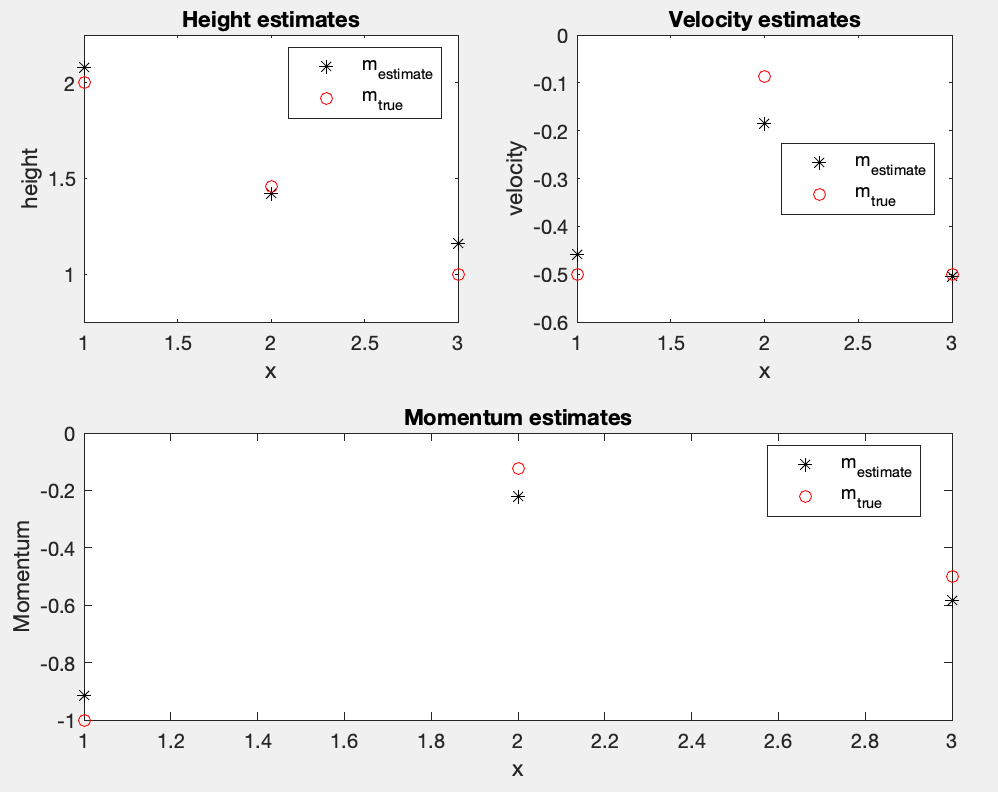
\includegraphics[width=1.0\linewidth]{estimates_15}
		\caption{}
		\label{fig:exap}
	\end{subfigure}
	%
	\begin{subfigure}[b]{0.517\textwidth}
		\centering
		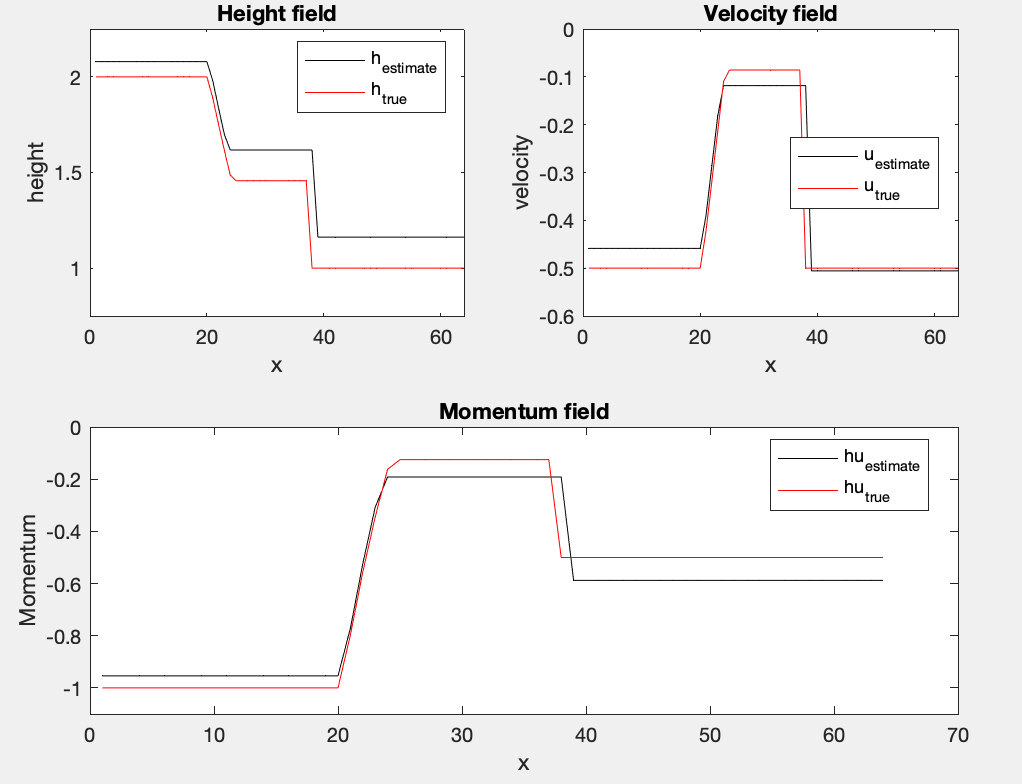
\includegraphics[width=1.0\linewidth]{field_15}
		\caption{}
		\label{fig:exapp}
	\end{subfigure}
	\caption{(a) and (b) respectively show the parameter estimates and their corresponding data}
\end{figure}

\begin{figure}[H]
	\begin{subfigure}[b]{0.5\textwidth}
		\centering
		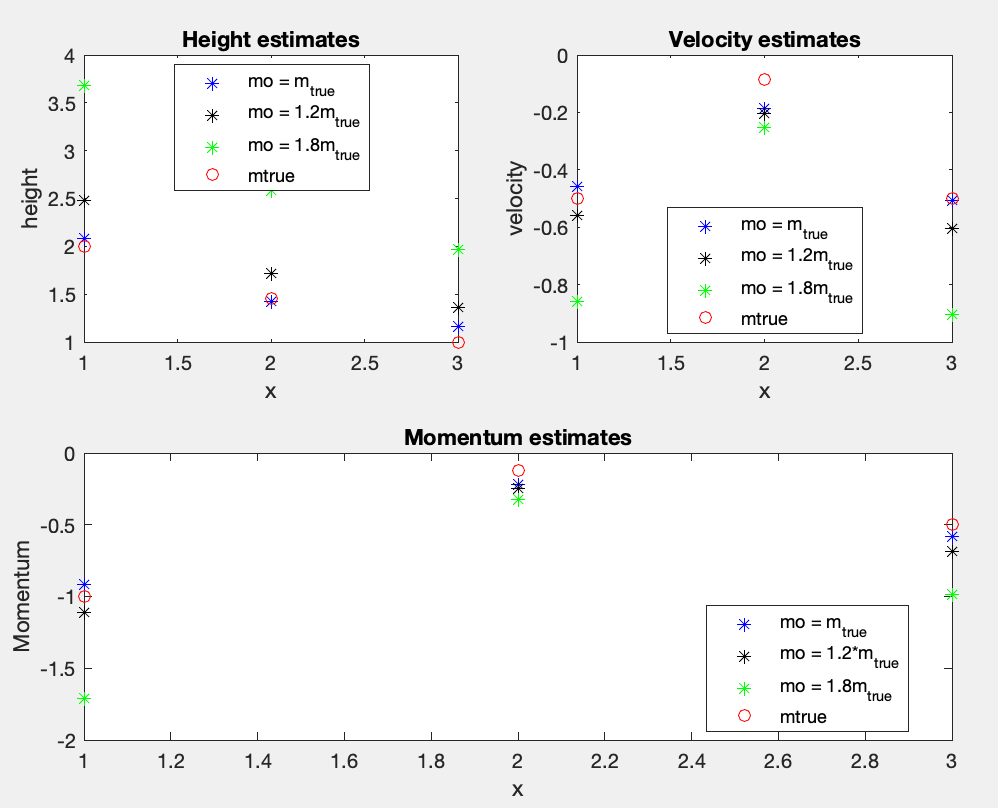
\includegraphics[width=1.0\linewidth]{comd}
		\caption{}
		\label{dd_mo}
	\end{subfigure}
	%
	\begin{subfigure}[b]{0.5\textwidth}
		\centering
		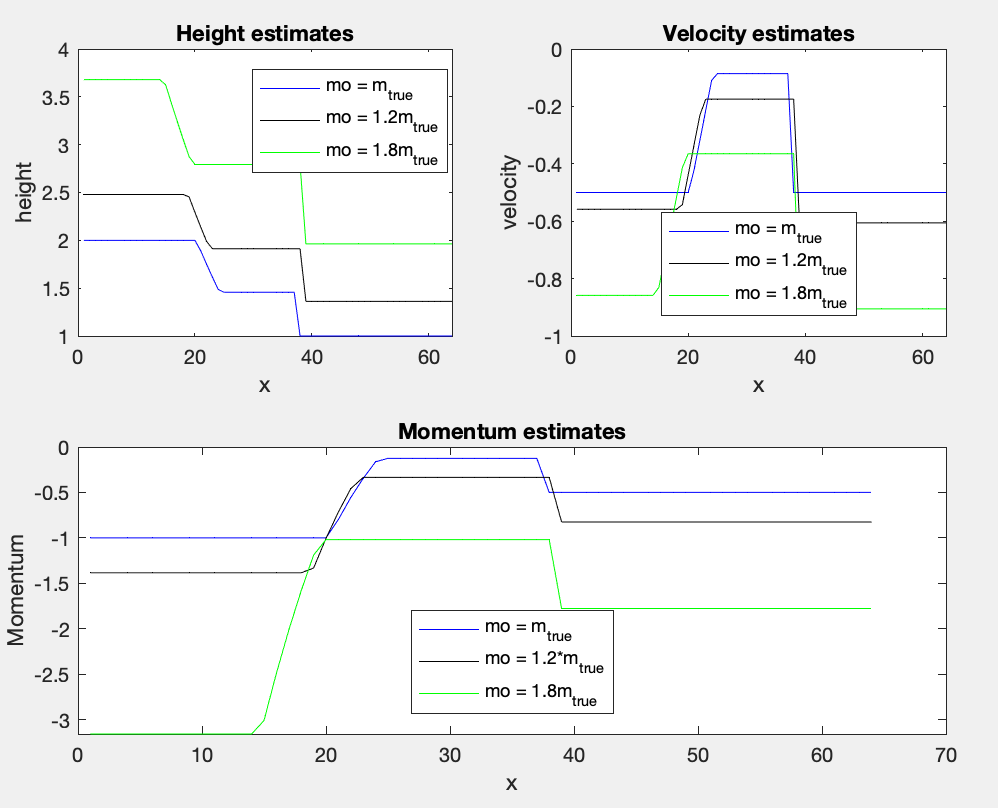
\includegraphics[width=1.0\linewidth]{ccom}
		\caption{}
		\label{dat}
	\end{subfigure}
	\caption{(a) and (b) respectively show the parameter estimates and their corresponding data based on the value of the initial estimates.}
\end{figure}
Figures~\ref{dd_mo} and \ref{dat} represents recovered estimates depending on the  initial estimates ($m_0$) used, 

explains how best we can choose the initial estimates ($m_0$) while recovering $m_{true}$. The closer $m_0$ is to $m_{true}$ 

	
			\begin{table}[H]
					\begin{center}
				\begin{tabular}{|c|c|c|c|}
					\hline
					& $m_0$ = $m_{true}$ & $m_0 = 1.2m_{true}$ & $m_0 = 1.8m_{true}$ \\
					\hline
					$h$ & 0.69264 & 0.0099329  &0 \\
					\hline
					$u$ &  0.97701& 0.90333 & 0.062386 \\
					\hline
					$hu$ & 0.94026 & 0.10929  & 0 \\
					\hline
				\end{tabular}
				\caption{ P-values of different values of $m_0$  }
			\end{center}
			\end{table}




	\begin{figure}[H]
	\centering
	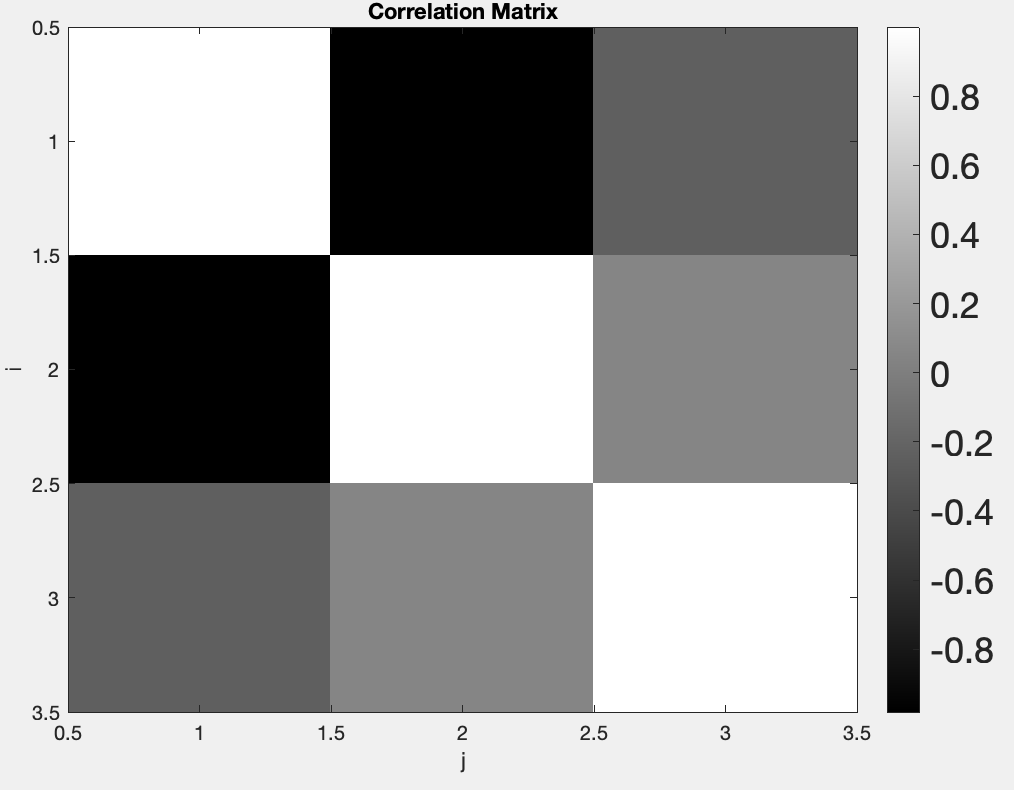
\includegraphics[width=0.5\linewidth]{correl}
	\caption{Correlation matrix }
	\label{cor}
\end{figure}
Figure.~\ref{cor}, displays the correlations between the recovered parameter estimates. 

\begin{equation}
	\text{Covariance matrix} = \begin{pmatrix}
		4.4814 & -4.4333	 & -0.2542 \\
		-4.4333 & 4.7621 & -0.0597 \\
		-0.2542 & -0.0597 & 0.3228
	\end{pmatrix}
\end{equation}

\begin{equation}
m_{true} = \begin{pmatrix}
		2.000& -0.500	 & -1.000 \\
		1.4571& -0.0858 & -0.1250 \\
		1.000 & -0.500 & -0.500
	\end{pmatrix}
\end{equation}

\begin{small}
	\begin{equation}
		C_h = \begin{pmatrix}
			-2.0528	 & 6.2456	 \\
			-2.7290& 5.5694 \\
			-2.9935 &5.3049
		\end{pmatrix}
		\quad
		C_u= \begin{pmatrix}
			-4.7359 & 3.8184	\\
			-4.4700 & 4.0844 \\
			-4.7801 & -3.7742
		\end{pmatrix}
		\quad
		C_{hu}= \begin{pmatrix}
			-2.0406 & 0.1867\\
			-1.3347 & 0.8927 \\
			-1.6924 & 0.5349
		\end{pmatrix}
	\end{equation}
\end{small}


\begin{equation}
\text{Correlation matrix} = \begin{pmatrix}
		1.0000 & -0.9597 & -0.2113 \\
		-0.9597 & 1.0000 & -0.0481 \\
		-0.2113 & -0.0481 & 1.0000
	\end{pmatrix}
\end{equation}


	\begin{figure}[H]
	\centering
	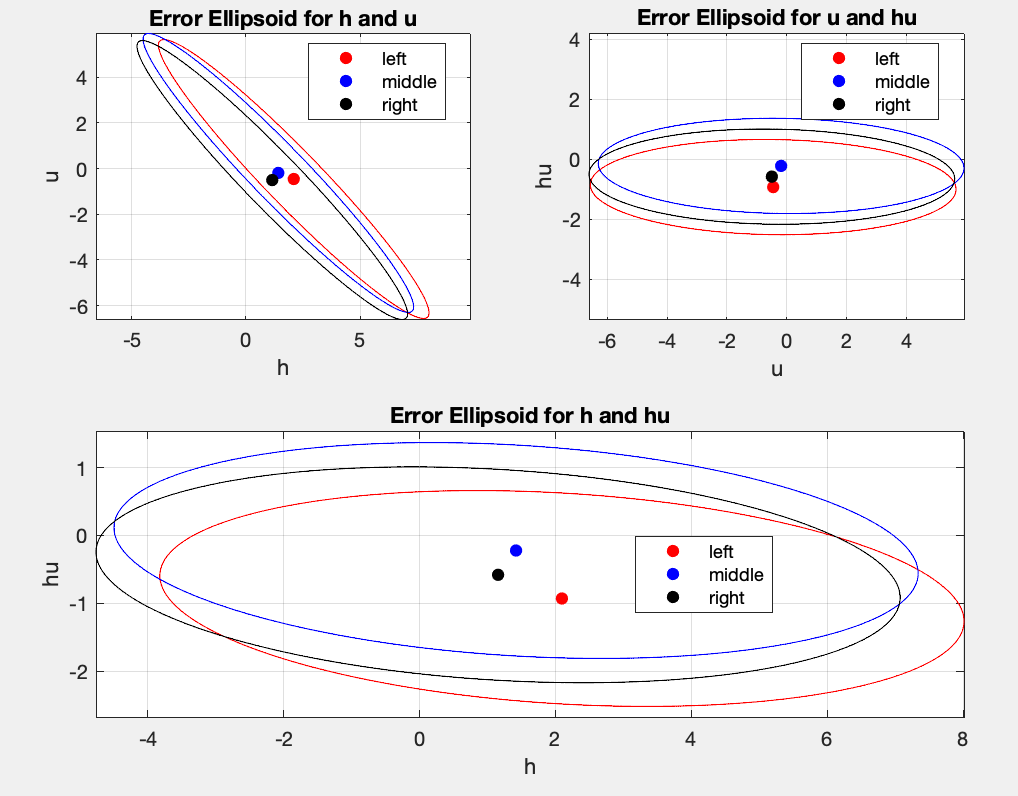
\includegraphics[width=0.5\linewidth]{error_ellipsoid}
	\caption{ Linear error ellipsiods }
	\label{err}
\end{figure}
Figure.~\ref{err}, contains three linear error ellipsoids depicting the confidence regions between parameters: $h$ and $u$, $u$ and $hu$, and h and $hu$ . The red, blue, and black dots represents the left, middle and right parameter estimates. Since these estimates lie at the center for each of the corresponding colour region, implies that the estimates lie with in the confidence regions.

	\begin{figure}[H]
	\centering
	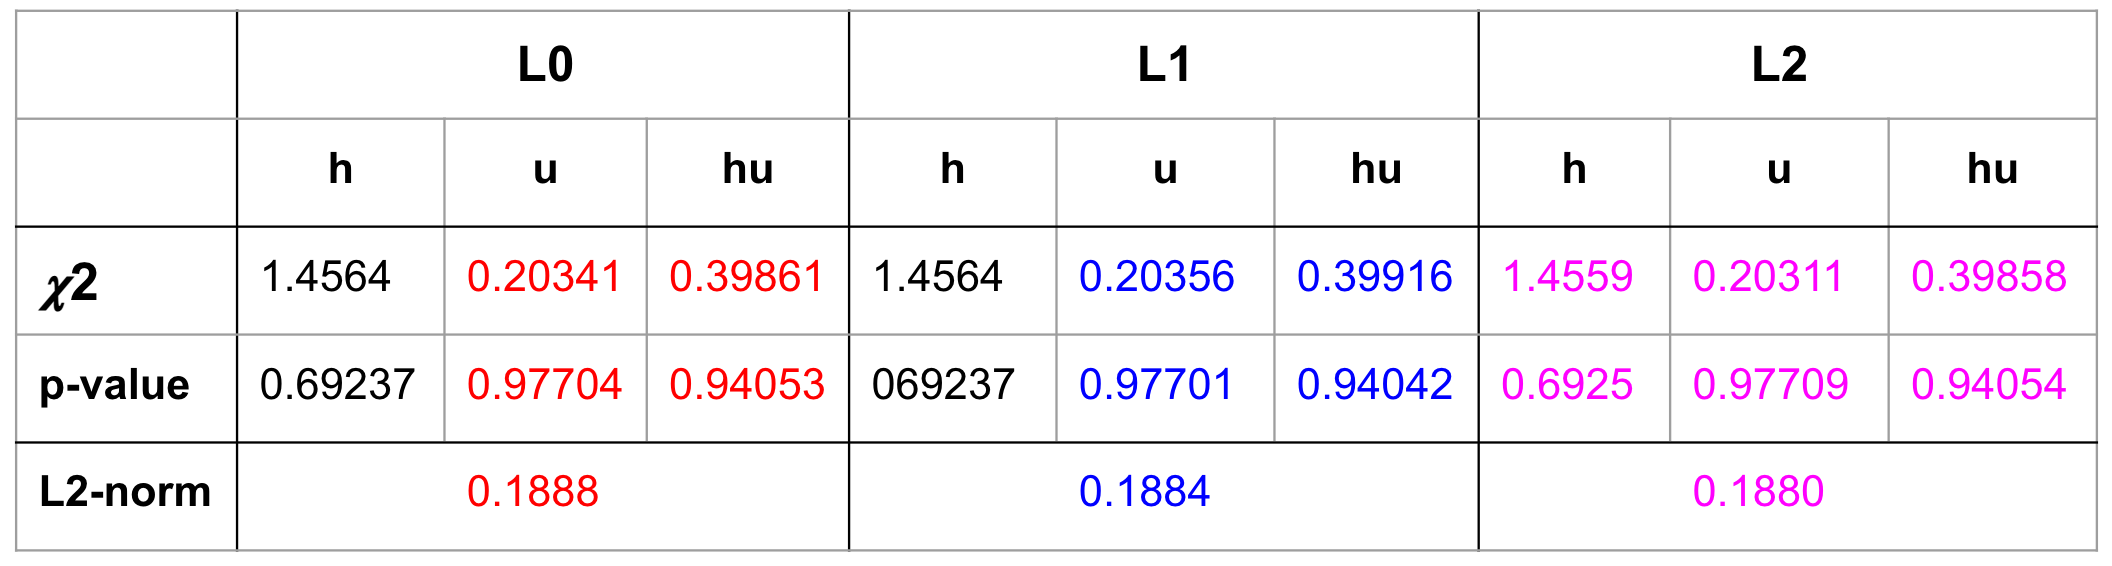
\includegraphics[width=0.5\linewidth]{con}
	\caption{ The Chi-square, p-value, and the L2-norm for the three roughening matrices: zeroth, first, and second. }
	\label{fig:confidence}
\end{figure}
	\section{Conclusion}
	I discovered that recovering mtrue, depends on:
	The initial estimate ,mo, used.
	The value of the standard deviation used to generate the noise.
	The step size ,h,
	The inversion model used which high depends on the range of values of alpha used.
	The order of  the roughening matrix used.
	P-value is highly affected by input parameters: tfinal, h, roughening matrix, inversion model, N, e.t.c.
	


	\bibliographystyle{abbrvnat}
\bibliography{document,geoclaw,literature}
	
	\section{Appendix}
	
	
	\subsection{Forestclaw solver}
	\begingroup\makeatletter\def\@currenvir{verbatim} 	\label{exact}
	\verbatim
	%%====================================================================
	% Boise State University
	% Author: Brian KYANJO
	% supervised by: Prof. Jodi Mead
	% class: Inverse Methods
	% Date: March 17th, 2022
	% final project
	%
	% Description:
	% -----------
	% Uses the Initial Riemann problem to find an intemediate state (qm) which either 
	% the intial left or right state connects to it via any combination of shocks and
	% rarefactions in the two families.
	% 
	% For Riemann problems with an initial dry state on one side, the exact Riemann 
	% solution contains only a single rarefaction connecting the wet to dry state.
	% The evolving wet dry interface is therefore simply one edge of the rarefaction. 
	% The propagation speed of this interface can be exactly determined using the 
	% Riemann invariants of the corresponding characteristics field.
	% 
	% Input:
	% -----
	% x  - array of spacial points 
	% t  - array of temporal points
	% mq - specifies the output (0 and 1 corresponds to h and hu respectively) 
	% ql - left initial state
	% qr - right initial state
	% Returns:
	% h  - array of hieght field values
	% hu - array of momentum field values
	%%=====================================================================
	
	% Exact solver
	function [Q,hs,us] = forestclaw(ql,qr,xi)
	global g; 
	hl = ql(1); hr = qr(1);
	ul = ql(2); ur = qr(2);
	
	hs = Newton(hl,hr,ul,ur);  %calling the newton solver
	us = ul - phi(hs,hl);
	
	if xi <= us
	if hs > hl
	s = ul - sqrt(0.5*g*hs/hl*(hl+hs));
	if xi <= s
	h = hl;
	hu = hl*ul;
	else
	h = hs;
	hu = hs*us;
	end
	else
	head = ul -sqrt(g*hl);
	tail = us - sqrt(g*hs);
	if xi <= head
	h = hl;
	hu = hl*ul;
	elseif xi >= tail
	h = hs;
	hu = hs*us;
	else
	h = (((ul + 2*sqrt(g*hl) - xi)/3)^2)/g;
	u = xi + sqrt(g*h);
	hu = h*u;
	end
	end
	else
	if hs > hr
	s = ur + sqrt(0.5*g*hs/hr*(hs+hr));
	if xi <=s
	h = hs;
	hu = hs*us;
	else
	h = hr;
	hu = hr*ur;
	end
	else
	head = ur + sqrt(g*hr);
	tail = us + sqrt(g*hs);
	if xi >= head
	h = hr;
	hu = hr*ur;
	elseif xi <= tail
	h = hr;
	hu = hr*ur;
	else
	h = (((xi-ur+2*sqrt(g*hr))/3)^2)/g;
	u = xi - sqrt(g*h);
	hu = h*u;
	end
	end
	end
	Q = [h;hu./h;hu];
	end
	
	% Newton solver
	function [hs] = Newton(hl,hr,ul,ur)
	global g;
	hs = ((sqrt(hl) + sqrt(hr) - (ur-ul)/2/sqrt(g))^2)/4;
	tol = 1e-12;
	max_iter = 100;
	
	for i=1:max_iter
	gk = func(hs,hl,hr,ul,ur);
	res = abs(gk);
	
	if (res<tol)
	break
	else
	continue
	end
	
	dg = dfun(hs,hl,hr,ul,ur);
	dh = -gk/dg;
	delta = 1;
	
	for i=1:500
	if (abs(func(hs+dh*delta,hl,hr,ul,ur)) >= res)
	delta = 0.5*delta;
	else
	break
	end
	end
	hs = hs + delta*dh;
	end
	end
	
	% phi function
	function [h] = phi(hs,hlr)
	global g; 
	if (hs>hlr)
	h = sqrt(0.5*g*(hs + hlr)/(hs*hlr))*(hs - hlr);
	else
	h = 2*sqrt(g)*(sqrt(hs) - sqrt(hlr));     
	end
	end
	
	% function f
	function [f] = func(hs,hl,hr,ul,ur)
	global g; 
	f = phi(hs,hl) + phi(hs,hr) + ur - ul;
	end
	
	% Jacobian of f
	function [df] = dfun(hs,hl,hr,ul,ur)
	global g; 
	eps = 1e-7;
	df = (func(hs+eps,hl,hr,ul,ur) - func(hs-eps,hl,hr,ul,ur))/(2*eps);
	end
	
	
	function plot_ellipse(DELTA2,C,m,first,second)
	n=5000;
	%first - first parameter
	%second - second parameter
	%construct a vector of n equally-spaced angles from (0,2*pi)
	theta=linspace(0,2*pi,n)';
	
	%corresponding unit vector
	xhat=[cos(theta),sin(theta)];
	Cinv=inv(C);
	
	%preallocate output array
	r=zeros(n,2);
	for i=1:n
	%store each (x,y) pair on the confidence ellipse in the corresponding row of r
	r(i,:)=sqrt(DELTA2/(xhat(i,:)*Cinv*xhat(i,:)'))*xhat(i,:);
	end
	
	% Plot the ellipse and set the axes.
	for i = 1:3
	a=['r' 'b' 'k'];
	plot(m(i,first)+r(:,1), m(i,second)+r(:,2),'color',a(i)); hold on
	plot(m(i,first),m(i,second),'.','color',a(i),'MarkerSize',17);grid on
	axis equal
	end
	end
\end{verbatim}

\subsection{Model}
\begingroup\makeatletter\def\@currenvir{verbatim}
\verbatim
%%====================================================================
% Author: Brian KYANJO
% supervised by: Prof. Jodi Mead
% class: Inverse Methods
% Date: March 17th, 2022
% final project
%  [Q] = model(m)
%
% INPUT
%   m - a guess at the model
%
% OUTPUT
%   Q   - a model matrix G(ql,qr,x/t) for the forward problem
%%====================================================================

function [Q] = model(m)
global N; global M; global h;
global t; global x;

for j= 2:M % time loop
for i=1:N % spartial loop
xi = x(i)/t(j);
[Q(:,i),hs,us] = forestclaw(m(1,:),m(3,:),xi);
end
end
Q = Q'; 

\end{verbatim}

\subsection{Jacobian}
\begingroup\makeatletter\def\@currenvir{verbatim}
\verbatim
%%====================================================================
% Boise State University
% Author: Brian KYANJO
% supervised by: Prof. Jodi Mead
% class: Inverse Methods
% Date: March 17th, 2022
% final project
%  [J] = Jacobian(m)
%
% INPUT
%   m - a guess at the model
%
% OUTPUT
%   J   - its corresponding Jacobian
%%====================================================================

function [J] = Jacobian(m)
global N; global M; global h;
global t; global x;

for j= 2:M % time loop
J = [];
for i=1:N % spartial loop
xi = x(i)/t(j);

% Formulation of Jacobian Matrix
ej = ones(3,1); 
[Qmin(:,i),hs,us] = forestclaw(m(1,:)-h*ej,m(3,:)-h*ej,xi);
[Qmax(:,i),hs,us] = forestclaw(m(1,:)+h*ej,m(3,:)+h*ej,xi);
J = [J (Qmax(:,i) - Qmin(:,i))./(2*h)]; % Jacobian
end
end
J = J';

\end{verbatim}

\subsection{Test  script}
\begingroup\makeatletter\def\@currenvir{verbatim}
\verbatim

%%====================================================================
% Boise State University
% Author: Brian KYANJO
% supervised by: Prof. Jodi Mead
% class: Inverse Methods
% Date: March 17th, 2022
% final project
% main_fuction script
%%=====================================================================
function main_function(mtrue,mo,h,L,x,ql,qr,M,t,mq)
global N; global sig;
hr = qr(1); hl = ql(1)
% Initial conditions
Q = zeros(3,N);
for i=1:N
if (x(i)<=0) 
Q(:,i) = ql;
else
Q(:,i) = qr;
end
end

% writing a video
v = VideoWriter('dam.avi');
open(v);

for j= 2:M % time loop
J = [];
for i=1:N % spartial loop
xi = x(i)/t(j);
[Q(:,i),hs,us] = forestclaw(ql,qr,xi);
end

noise = sig*randn(size(Q(:,:)));      % genrate noise
d = Q(:,:) + noise;   d = d';         % add noise to the data

dh = d(:,1); du = d(:,2); dhu = d(:,3);
dnoise = [0.005*dh  0.005*du 0.005*dhu ];
d = Q(:,:) + dnoise';

d = d';                               % transposing data d
delta = sig*sqrt(N);                  % delta
fun = @(m) model(m);                  % model function handle
jac = @(m) Jacobian(m);               % Jacobian function handle

m = occam(fun, jac, L, d, mo, delta);    % calling the Occam model to  recover mtrue

% plotting estimates
figure(1)
if mq == 1
plot(m(:,mq),'k*'); hold on
plot(mtrue(:,mq),'ro'); hold off
legend('m_{estimate}','m_{true}',Location='best')
title('Height field');
ylim([hr-0.25,hl+0.25]);
ylabel('height');xlabel('x')
frame = getframe(gcf);
writeVideo(v,frame);
elseif mq == 2
plot(m(:,mq),'k*'); hold on
plot(mtrue(:,mq),'ro'); hold off
legend('m_{estimate}','m_{true}',Location='best')
title('velocity field')
ylabel('velocity');xlabel('x')
frame = getframe(gcf);
writeVideo(v,frame);
elseif mq == 3
plot(m(:,mq),'k*'); hold on
plot(mtrue(:,mq),'ro'); hold off
legend('m_{estimate}','m_{true}',Location='best')
title('momentum field')
ylabel('Momentum');xlabel('x')
frame = getframe(gcf);
writeVideo(v,frame);
else
subplot(2,2,1)
plot(m(:,1),'k*'); hold on
plot(mtrue(:,1),'ro');  hold off
legend('m_{estimate}','m_{true}',Location='best')
title('Height estimates')
ylim([hr-0.25,hl+0.25])
ylabel('height');xlabel('x')
subplot(2,2,2);
plot(m(:,2),'k*'); hold on
plot(mtrue(:,2),'ro'); hold off
legend('m_{estimate}','m_{true}',Location='best')
title('Velocity estimates')
ylabel('velocity');xlabel('x')
subplot(2,2,[3,4]);
plot(m(:,3),'k*'); hold on
plot(mtrue(:,3),'ro'); hold off
title('Momentum estimates')
ylabel('Momentum');xlabel('x')
legend('m_{estimate}','m_{true}',Location='best')
frame = getframe(gcf);
writeVideo(v,frame);
end

for i=1:N 
xi = x(i)/t(j);
[Qest(:,i),hs,us] = forestclaw(m(1,:),m(3,:),xi);
end

% chi-square
chi_s = zeros(3,1); ad = d';
for k = 1:N
chi_s = chi_s + (Qest(:,k) - ad(:,k)).^2;   
end

% pvalue
dof = N - 9; %degrees of freedom
p = 1 - chi2cdf(chi_s,3);

% plotting data
figure(2)
if mq == 1
plot(Qest(mq,:),'k'); hold on
plot(Q(mq,:),'r'); hold off
legend('h_{estimate}','h_{true}',Location='best')
title('Height field');
ylim([hr-0.5,hl+0.5]);
ylabel('height');xlabel('x')
frame = getframe(gcf);
writeVideo(v,frame);
elseif mq == 2
plot(Qest(mq,:),'k'); hold on
plot(Q(mq,:),'r'); hold off
legend('u_{estimate}','u_{true}',Location='best')
title('velocity field')
ylabel('velocity');xlabel('x')
frame = getframe(gcf);
writeVideo(v,frame);
elseif mq == 3
plot(Qest(mq,:),'k'); hold on
plot(Q(mq,:),'r'); hold off
legend('hu_{estimate}','hu_{true}',Location='best')
title('momentum field')
ylabel('Momentum');xlabel('x')
frame = getframe(gcf);
writeVideo(v,frame);
else
subplot(2,2,1)
plot(Qest(1,:),'k'); hold on
plot(Q(1,:),'r'); hold off
legend('h_{estimate}','h_{true}',Location='best')
title('Height field')
ylim([hr-0.25,hl+0.25])
ylabel('height');xlabel('x')
subplot(2,2,2);
plot(Qest(2,:),'k'); hold on
plot(Q(2,:),'r'); hold off
legend('u_{estimate}','u_{true}',Location='best')
title('Velocity field')
ylabel('velocity');xlabel('x')
subplot(2,2,[3,4]);
plot(Qest(3,:),'k'); hold on
plot(Q(3,:),'r'); hold off
ylim([-1.1,0])
title('Momentum field')
ylabel('Momentum');xlabel('x')
legend('hu_{estimate}','hu_{true}',Location='best')
frame = getframe(gcf);
writeVideo(v,frame);

end


%Covariance Matrix
J = Jacobian(m); 
C = inv(J'*J);

%confidence interval
za = 1.96; % 95% confidence interval

% first parameter
s1 = sqrt(C(1,1)); % standard deviation
s2 = sqrt(C(2,2));
s3 = sqrt(C(3,3));

% confidence intervals 
c1 = m(:,1)- za*s1;
c2 = m(:,1) + za*s1;
c11 = m(:,2)- za*s2;
c22 = m(:,2) + za*s2;
c13 = m(:,3)- za*s3;
c33 = m(:,3) + za*s3;

%Correlation matrix
rho11 = C(1,1)/sqrt(C(1,1)*C(1,1));
rho22 = C(2,2)/sqrt(C(2,2)*C(2,2));
rho33 = C(3,3)/sqrt(C(3,3)*C(3,3));
rho12 = C(1,2)/sqrt(C(1,1)*C(2,2));
rho13 = C(1,3)/sqrt(C(1,1)*C(3,3));
rho23 = C(2,3)/sqrt(C(2,2)*C(3,3));
Correlation_matrix = [rho11 rho12 rho13;rho12 rho22 rho23;...
rho13 rho23 rho33];


end
close(v);

disp(['chi-square obs = [',num2str(chi_s'),']'])
disp(['pvalue = [',num2str(p'),']'])
L2norm = norm(mtrue - m,2)
mtrue
covariance_matrix = C
cofidence_interval_height = [c1 c2]
cofidence_interval_velocity = [c11 c22]
cofidence_interval_Momentum = [c13 c33]

Correlation_matrix = Correlation_matrix


%Linearised ellipsoid
Delta = chi2inv(0.95,3); %Delta2

figure(4)
subplot(2,2,1)
plot_ellipse(Delta,C(1:2,1:2),m,1,2); 
grid on
title('Error Ellipsoid for h and u')
legend('','left','','middle','','right',Location='best')
xlabel('h'); ylabel('u')
subplot(2,2,2)
C1 = [C(2,2) C(2,3); C(3,2) C(3,3)];
plot_ellipse(Delta,C1,m,2,3); 
grid on
title('Error Ellipsoid for u and hu')
legend('','left','','middle','','right',Location='best')
xlabel('u'); ylabel('hu')
subplot(2,2,[3,4]);
C2 = [C(1,1) C(1,3); C(3,1) C(3,3)];
plot_ellipse(Delta,C2,m,1,3); 
grid on
title('Error Ellipsoid for h and hu')
legend('','left','','middle','','right',Location='best')
xlabel('h'); ylabel('hu')

Corr = corrcoef(C);

figure(7)
clf
colormap('gray')

imagesc(Corr)
set(colorbar,'Fontsize',18);
xlabel('j')
ylabel('i')
title('Correlation Matrix')
end


\end{verbatim}

\subsection{Main script}
	\begingroup\makeatletter\def\@currenvir{verbatim}
\verbatim
%%====================================================================
% Boise State University
% Author: Brian KYANJO
% supervised by: Prof. Jodi Mead
% class: Inverse Methods
% Date: March 17th, 2022
% final project
% main script
%%=====================================================================

clc
clear
close all

global g; global N;
global sig; global h;
global t; global x;
global M;
warning('off','all')

% problem
hl = 2;                          % left depth
hr = 1;                          % right depth
ul = -0.5;                       % left velocity
ur = -0.5;                       % right velocity

% Spatial domain
ax = -5;
bx = 5;
ay = -2;
by = 4;
meqn = 2;                       % Number of equations in the system


g = 1;                          % Gravity 

to = 0;                         % initial time
Tfinal = 1;                     % final time

ql = [hl; ul; hl*ul];           % left conservation variable
qr = [hr; ur; hr*ur];           % right consrvation variable
qm = [(hl+hr)/2 (ul+ur)/2 ...   % intermediate initial state
(hl*ul+hr*ur)/2];

N = 64;                         % Number of spartial steps

dx = (bx - ax)/N;               % spartial step size

cfl = 0.9;                      % cfl number

a = 1.5;                        % maximum velocity

dt_est = cfl*dx/a;

M = (floor(Tfinal/dt_est) + 1); % number of time steps

dt = Tfinal/(M);                % temporal step size

t = linspace(to,Tfinal,M);      % temporal domain

xe = linspace(ax,bx,N+1);       % edge locations
x = xe(1:end-1) + dx/2;         % Cell-center locations

mq = 4;                         % 1-height, 
% 2-velocity, 
% 3-momentum, 
% 4-all fields
h = 0.9;

sig = 1e-3;                     % standard deviation

L0 = eye(3);          % generate roughening matrices
L1 = get_l_rough(3,1);
L2 = get_l_rough(3,2); 


qll = [hl ul hl*ul];            % left conservation variable
qrr = [hr ur hr*ur];            % right conservation variable
xi = x(1)/t(2);                 % initial speed
[Q(:,1),hs,us] = forestclaw(ql,qr,xi); % initial conservation variable
qmm = [hs us hs*us];                   % intermediate state
%mo = [qll;qm;qrr];
mtrue = [qll; qmm; qrr];               % true parameters

mo = 1.5*mtrue;
main_function(mtrue,mo,h,L0,x,ql,qr,M,t,mq) %calling the main function script



\end{verbatim}

\end{document}